\documentclass{article}
\usepackage[utf8]{inputenc}
\usepackage[none]{hyphenat}
\usepackage[a4paper, total={7in, 8.5in}]{geometry}
\usepackage{graphicx}
\usepackage{amsmath}
\usepackage{amssymb}
\usepackage{mathtools}
\usepackage{bbm}
\usepackage{amsthm}
\usepackage{mathdots}
\usepackage{fancyhdr}
\usepackage[parfill]{parskip}
\usepackage{tikz}
\usepackage{subcaption}
\usepackage{hyperref}
\usepackage{minted}
\theoremstyle{definition}
\newtheorem{theorem}{Theorem}
\newtheorem{definition}{Definition}
\newtheorem{example}{Example}
\newenvironment{theoremqed}
    {\begin{theorem}}
    {\hfill \qedsymbol \end{theorem}}
\newenvironment{definitionqed}
    {\begin{definition}}
    {\hfill \qedsymbol \end{definition}}
\newenvironment{exampleqed}
    {\begin{example}}
    {\hfill \qedsymbol \end{example}}

\renewcommand{\qedsymbol}{\(\blacksquare\)}
\newcommand{\X}{\mathbf{X}}
\renewcommand{\P}{\mathbb{P}}

\setlength{\parskip}{2mm}

\begin{document}

\begin{titlepage}
    \centering
    \vspace*{3cm}
    {\huge \bfseries Bayesian Network with Discrete Random Variables and its Python Implementation \par}
    \vspace{5cm}
    {\Large Yuwei (Johnny) Meng \par}
    \vspace{3cm}
    {\large Department of Statistical Sciences, University of Toronto}
    \vfill
\end{titlepage}

\tableofcontents

\pagebreak

\section{Preface \& Acknowledgements}

\pagebreak

\section{Bayesian Network}

\subsection{Motivation}

Consider a set of random variables \(\X = (X_1, \cdots, X_n)\) where each \(X_i\in \{x_i, \neg x_i\}\) is binary. To specify the joint distribution of \(\X\), we need to list out all the possible combinations:
\begin{align*}
    &\P(x_1, x_2, \cdots, x_n); \\
    &\P(\neg x_1, x_2, \cdots, x_n); \\
    &\P(x_1, \neg x_2, \cdots, x_n); \\
    &\vdots
\end{align*}
For \(n\) random variables, the number of joint probabilities is \(2^n - 1\), which quickly becomes intractable as \(n\) grows large, requiring a more efficient framework for modeling joint probabilities. Bayesian Network, or Directed Acyclic Graphical Model (DAGM), is one such framework exploiting \textit{Theorem \ref{thm:chain_rule}} below.

\begin{theoremqed} \label{thm:chain_rule}
    \textbf{(Chain Rule of Probability)} Let \(X_1, \cdots, X_n\) be random variables. Then the joint probability can be expressed as
    \begin{align*}
        \P(X_1, \cdots, X_n) &= \P(X_1) \P(X_2, X_3, \cdots, X_n | X_1) \\
        &= \P(X_1) \P(X_2 | X_1) \P(X_3, \cdots, X_n | X_1, X_2) \\
        &= \cdots \\
        &= \P(X_1) \P(X_2 | X_1) \P(X_3 | X_1, X_2) \cdots \P(X_n | X_1, X_2, \cdots, X_{n-1}) \\
        &= \prod_{i=1}^n \P(X_i | X_1, X_2, \cdots, X_{i-1}).
    \end{align*}
\end{theoremqed}

Thus, if we have prior knowledge about the conditional independence relationships between the random variables we are modeling, then we can express the joint distribution in a more compact form, which motivates the use of Bayesian Networks.

\subsection{Introduction to Bayesian Network}

An example of Bayesian Network is shown in \textit{Figure \ref{fig:bayesian_network}} below.

\begin{figure}[htbp]
    \centering
    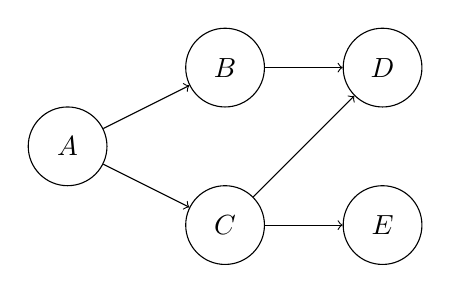
\begin{tikzpicture}
        \node[circle, draw, minimum size=1cm] (A) at (0,0) {\(A\)};
        \node[circle, draw, minimum size=1cm] (B) at (2,1) {\(B\)};
        \node[circle, draw, minimum size=1cm] (C) at (2,-1) {\(C\)};
        \node[circle, draw, minimum size=1cm] (D) at (4,1) {\(D\)};
        \node[circle, draw, minimum size=1cm] (E) at (4,-1) {\(E\)};

        \draw[->] (A) -- (B);
        \draw[->] (A) -- (C);
        \draw[->] (B) -- (D);
        \draw[->] (C) -- (D);
        \draw[->] (C) -- (E);
    \end{tikzpicture}
    \caption{Bayesian Network Example}
    \label{fig:bayesian_network}
\end{figure}

In this Bayesian Network, each vertex represents a random variable. The arrows denote conditional dependencies between random variables. For example, the edge \(A \longrightarrow B\) implies that \(B\) is directly conditionally dependent on \(A\). With this structure, we can model the joint distribution of these random variables in the following way:

\begin{definitionqed} \label{def:bayesian_network}
    Let \(\X = (X_1, \cdots, X_n)\) be a set of random variables modeled by a Bayesian Network. Then the joint probability can be expressed as
    \[\P(X_1, \cdots, X_n) = \prod_{i=1}^n \P(X_i | \operatorname{Parents}(X_i)).\]
\end{definitionqed}

\begin{exampleqed} \label{ex:bayesian_network}
    For the Bayesian Network shown in \textit{Figure \ref{fig:bayesian_network}}, the joint probability can be expressed as
    \[\P(A, B, C, D, E) = \P(A)\cdot\P(B|A)\cdot\P(C|A)\cdot\P(D|B,C)\cdot\P(E|C).\]
\end{exampleqed}

Note that \textit{Definition \ref{def:bayesian_network}} is a special case of \textit{Theorem \ref{thm:chain_rule}}, given that we have prior knowledge of the conditional independence relationships between the random variables. As a result, we can reduce the number of conditionals in the product and express the joint distribution in a more compact form. To illustrate this concept more clearly, let's define some probabilities for the Bayesian Network shown in \textit{Figure \ref{fig:bayesian_network}}. These probabilities will be used throughout the rest of this document.

\begin{exampleqed} \label{ex:bayesian_network_prob}
    Let \(A, B, C, D, E \in \{0, 1\}\) be binary random variables with the following conditional probabilities:

    \begin{figure}[htbp]
        \centering
        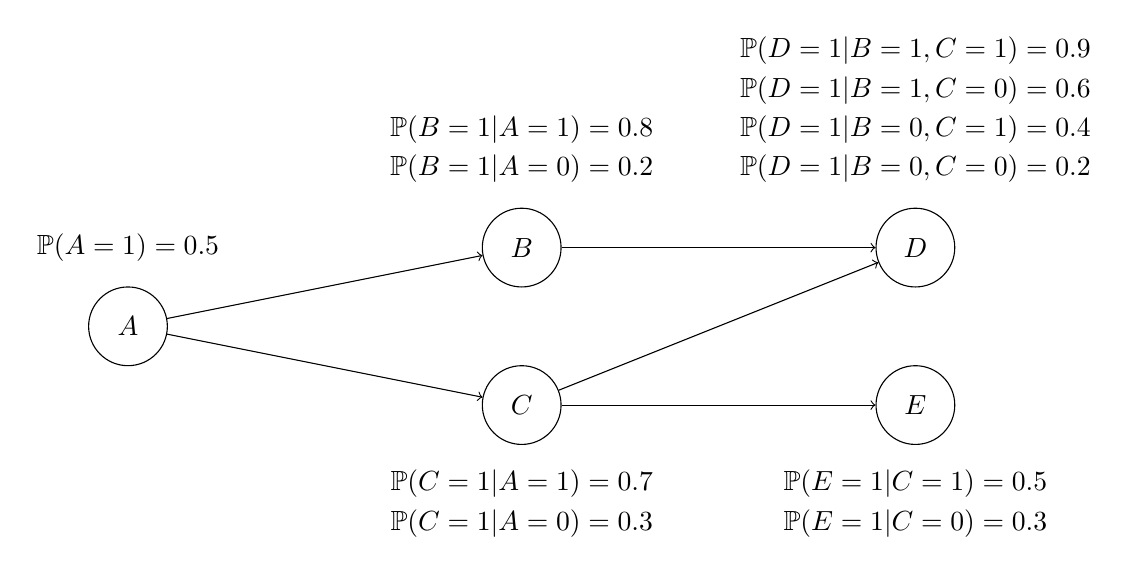
\begin{tikzpicture}
            \node[circle, draw, minimum size=1cm] (A) at (0,0) {\(A\)};
            \node[circle, draw, minimum size=1cm] (B) at (5,1) {\(B\)};
            \node[circle, draw, minimum size=1cm] (C) at (5,-1) {\(C\)};
            \node[circle, draw, minimum size=1cm] (D) at (10,1) {\(D\)};
            \node[circle, draw, minimum size=1cm] (E) at (10,-1) {\(E\)};
    
            \node (P_A) at (0,1) {\(\P(A=1)=0.5\)};
            \node (P_B_A1) at (5,2.5) {\(\P(B=1|A=1)=0.8\)};
            \node (P_B_A0) at (5,2) {\(\P(B=1|A=0)=0.2\)};
            \node (P_C_A1) at (5,-2) {\(\P(C=1|A=1)=0.7\)};
            \node (P_C_A0) at (5,-2.5) {\(\P(C=1|A=0)=0.3\)};
            \node (P_D_B1_C1) at (10,3.5) {\(\P(D=1|B=1,C=1)=0.9\)};
            \node (P_D_B1_C0) at (10,3) {\(\P(D=1|B=1,C=0)=0.6\)};
            \node (P_D_B0_C1) at (10,2.5) {\(\P(D=1|B=0,C=1)=0.4\)};
            \node (P_D_B0_C0) at (10,2) {\(\P(D=1|B=0,C=0)=0.2\)};
            \node (P_E_C1) at (10,-2) {\(\P(E=1|C=1)=0.5\)};
            \node (P_E_C0) at (10,-2.5) {\(\P(E=1|C=0)=0.3\)};
    
            \draw[->] (A) -- (B);
            \draw[->] (A) -- (C);
            \draw[->] (B) -- (D);
            \draw[->] (C) -- (D);
            \draw[->] (C) -- (E);
        \end{tikzpicture}
        \caption{Bayesian Network with Probabilities Example}
        \label{fig:bayesian_network_probs}
    \end{figure}
\end{exampleqed}

Note that only 11 conditional probabilities are needed to specify the joint distribution of the 5 random variables in our Bayesian Network, which is a significant improvement compared to the \(2^5 - 1 = 31\) joint probabilities in the general case. The exact number of required conditional probabilities depends on the structure of the Bayesian Network, though, but as long as there are some conditional independence relationships between the random variables, we can always expect a reduction in the number of required conditional probabilities.

\subsection{Implementation}

The implementation of Bayesian Network in this project consists of multiple modules which are discussed separately in the following subsections.

\subsubsection{\texttt{Distribution}}

The \texttt{distribution.py} file defines an abstract class called \texttt{Distribution}, as well as two inherited classes named \texttt{UnconditionalDistribution} and \texttt{ConditionalDistribution}. The purpose of these classes is to provide a data structure that encodes the probability distribution of a vertex in the Bayesian Network.

The abstract class \texttt{Distribution} has the attribute and method definitions:

\begin{minted}{python}
    domain: set
\end{minted}

This attribute defines the set of possible values for the random variables.

\begin{minted}{python}
    __call__(self, *args) -> float
\end{minted}

This method evaluates the probability of the random variable taking on a specific value in the domain.

\subsubsection{\texttt{UnconditionalDistribution}}

The \texttt{UnconditionalDistribution} class defines the distribution of a random variable that does not have a parent in the Bayesian Network, as well as the distribution of a random variable conditioned on its parents. Besides the inherited attribute \texttt{domain}, it has the following attribute:

\begin{minted}{python}
    distribution: dict[Any, float]
\end{minted}

This attribute serves as a lookup table for the unconditional distribution of the random variable. The keys of the dictionary are the possible values of the random variable, and the values are the corresponding probabilities.

This class also implements the \texttt{\_\_call\_\_} method. The expected argument is a value in the domain of the random variable, and the method outputs the probability of the random variable taking on that value. If the argument is not in the domain, a \texttt{ValueError} will be raised.

\begin{exampleqed}
    For the Bayesian Network shown in \textit{Figure \ref{fig:bayesian_network_probs}}, the distribution of vertex \(A\) would have the following behaviors:

    \begin{minted}{python}
        >>> dist_A = UnconditionalDistribution(domain={0, 1}, distribution={0: 0.5, 1: 0.5})
        >>> dist_A(0)
        0.5
        >>> dist_A(1)
        0.5
    \end{minted}
\end{exampleqed}

\subsubsection{\texttt{ConditionalDistribution}}

This class defines the distribution of a random variable that has parents in the Bayesian Network. It inherits the \texttt{domain} attribute from the \texttt{Distribution} class, and it has the following attributes:

\begin{minted}{python}
    distributions[frozenset[str], UnconditionalDistribution]
\end{minted}

The keys of this dictionary are \texttt{frozenset}s of conditionals of the random variable, and the values define the distribution of the random variable conditioned on the values of its parents. 

This class also implements the \texttt{\_\_call\_\_} method. The expected arguments are a value in the domain of the random variable and a dictionary of the values of its parents. The method outputs the probability of the random variable taking on that value, given the values of its parents. If the value is not in the domain, or if the parents are not in the dictionary, or if the conditioning values are not in the domain of the parents, a \texttt{ValueError} will be raised.

This is slightly confusing, so the following example illustrates this concept.

\begin{exampleqed}
    For the Bayesian Network shown in \textit{Figure \ref{fig:bayesian_network_probs}}, the distribution of vertex \(D\) would have the following behaviors:

    \begin{minted}{python}
        >>> dist_D_B1C1 = UnconditionalDistribution(domain={0, 1}, distribution={0: 0.1, 1: 0.9})
        >>> dist_D_B1C0 = UnconditionalDistribution(domain={0, 1}, distribution={0: 0.4, 1: 0.6})
        >>> dist_D_B0C1 = UnconditionalDistribution(domain={0, 1}, distribution={0: 0.6, 1: 0.4})
        >>> dist_D_B0C0 = UnconditionalDistribution(domain={0, 1}, distribution={0: 0.8, 1: 0.2})
        >>> dist_D = ConditionalDistribution(domain={0, 1}, distributions={
            frozenset({'B: 1', 'C: 1'}): dist_D_B1C1,
            frozenset({'B: 1', 'C: 0'}): dist_D_B1C0,
            frozenset({'B: 0', 'C: 1'}): dist_D_B0C1,
            frozenset({'B: 0', 'C: 0'}): dist_D_B0C0
        })
        >>> dist_D(1, {'B': 1, 'C': 0})
        0.6
        >>> dist_D(0, {'C': 0, 'B': 0})
        0.8
    \end{minted}
\end{exampleqed}

The use of a \texttt{frozenset} data structure is a compromise to the need for a hashable data structure. The advantage is that we don't need to memorize the order of the parents when we are looking up the distribution because there is no inherent order for a \texttt{set} object. When looking up probabilities, the order in which we pass in the parents thus does not matter, as long as the values are correct, which ensures the efficiency of the lookup process.

\pagebreak

\section{Variable Elimination}

\end{document}